\chapter{Conceito do Sistema}
\label{chap:concep}
A percepção é, de acordo com o dicionário \citeonline{perc_michaelis}, a capacidade de distinguir por meio dos sentidos ou da mente.

Segundo \citeonline{chuck}, este é o ponto fraco mais comuns em robôs pois para garantir sua segurança e confiabilidade é necessário que o mesmo tenha a capacidade de interpretar as variáveis ambientais. A percepção é o que torna os robôs diferentes de simples mecanismos, pois é ela quem dá a habilidade de adequar suas operações de acordo com as influências externas.

A percepção do ELIR pode ser definida como um sistema integrado de sensoriamento e com unidades de processamento, em que seus dados serão utilizados como parâmetros de tomada de decisão e disponibilizados durante a operação de inspeção ao operador.

O sistema foi projetado de forma a possuir três subsistemas principais: segurança, georreferenciamento e detecção. A descrição de cada um dos subsistemas e suas funcionalidades serão mostradas nas próximas sessões.

\begin{flushright}
   \begin{list}{}{
      \setlength{\leftmargin}{4.5cm}
      \setlength{\rightmargin}{0cm}
      \setlength{\labelwidth}{0pt}
      \setlength{\labelsep}{\leftmargin}}
      \item Para um robô, o ambiente é um mar de ambiguidades, no qual ele vai afundar ou nadar a depender da robustez de sua percepção.


      \begin{list}{}{
      \setlength{\leftmargin}{0cm}
      \setlength{\rightmargin}{0cm}
      \setlength{\labelwidth}{0pt}
      \setlength{\labelsep}{\leftmargin}}
      \item \cite{Fitzpatrick}
      \end{list}
   \end{list}
\end{flushright}

%--------- NEW SECTION ----------------------
\section{Estudo do estado da arte}
\label{sec:sota}
flkjasdlkfjasdlkfjs

%--------- NEW SECTION ----------------------
\section{Descrição do sistema}
\label{sec:desc}
lasdjflsadjf

\subsection{Especificação técnica}
\label{ssec:espt}

A construção do sistema de Percepção teve como base os requisitos técnicos do cliente. As especificações podem ser observadas abaixo.
\begin{itemize}
\item O sistema foi projetado para trabalhar com alimentação de 14V proveniente de baterias LiPo.
\item A máxima temperatura de trabalho na \textit{housing} é de 50 graus Celsius.
\item O sistema consegue detectar objetos através do sonar em uma faixa de servidão de 6.45 metros.
\item A obtenção de \textit{frames} da câmera IR acontece na taxa de 1 frame a cada dois segundos.
\item Em condições de sobretemperatura ou sobrecorrente o sistema alertará o operador.
\item O sistema não é protegido contra ingresso de água
\end{itemize} 

\subsection{Arquitetura geral do sistema}
\label{ssec:arqg}
lkasjdflksdajflk;

\subsection{Arquitetura de software}
\label{ssec:arqs}


A arquitetura de software foi projetada em três camadas a fim de facilitar o desenvolvimento do sistema e simplificar o entendimento do mesmo. As camadas de são:

\begin{itemize}
	\item \textit{User Interface Layer}
	\item \textit{Business Layer}
	\item \textit{Drvier Layer}
\end{itemize}
 
As camadas e seus componentes podem ser vistos na Fig.\ref{arqsoft}.

\begin{figure}[H]
	\centering
	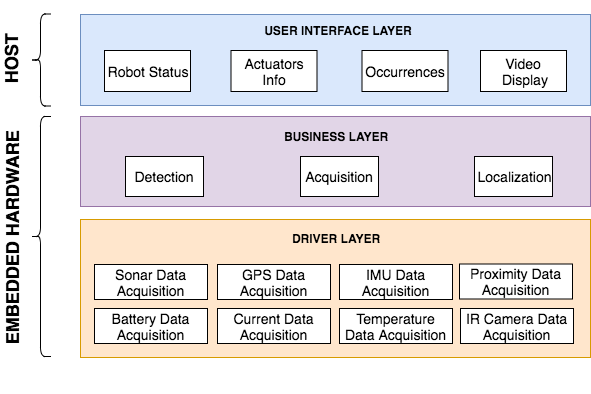
\includegraphics[width=15cm]{Figures/ArquiteturadeSoftware.png}
	\caption{Arquitetura Geral da Perception}
	\label{arqsoft}
\end{figure}

\subsubsection{Driver Layer}
	
A camada de \textit{Driver Layer} está diretamente relacionada a funcionalidade de aquisição de dados. Ela composta pelo \textit{hardware}, representado pelos sensores e seus respectivos drivers de comunicação. Desta forma, as subcamadas são nomeadas com o processo de aquisição de dados de cada sensor envolvido no projeto.

As subcamadas \textit{Current Data Acquisition}, \textit{Temperatura Data Acquisition}, \textit{Proximity Data Acquisition} e \textit{Sonar Data Acquisition} são responsáveis por adquirir as informações analógicas de seus sensores e transformá-los em dados da grandeza física a ser medida. Todas estas subcamadas utilizam a placa de interfaceamento Phidgets para o estabeler de comunicação entre o computador (NUC) e os sensores.

As subcamadas \textit{IMU Data Acquisition} e \textit{GPS Data Acquisition} são responsáveis pelo recebimento de dados da IMU e do GPS seguindo o protocolo de comunicação do fabricante. Esses dois módulos estão conectados ao HUB USB da placa de interfaceamente Phidgets. 

A subcamada de \textit{IR Camera Data Acquisition} é responsável pela aquisição de dados da câmera térmica, a qual se comunica via VOSPI com um microcontrolador de arquitetura ARM (STM32F401RE) e converte os dados para USB para a NUC. 
Por último, a subcamada de \textit{Battery Data Acquisition} é responsável pelo estabelecimento da comunicação e coleta de informações com o \textit{Smart Charger} de bateria utilizando protocolo SMBUS.

As conexões e diagramas elétricos podem ser vistos no apêndice \ref{Append:diagele}.

\subsubsection{Business Layer}

A camada \textit{business layer} é responsável por implementar a regra de negócio do sistema. As funcionalidades do sistema são representadas como sub-camadas da business layer, pois são elas responsáveis pelo processamento e coordenação dos dados adquiridos pela camada de aquisição.

\subsubsection{User Interface Layer}

A camada de \textit{User Interface} foi projetada para disponibilizar os dados para o operador. Nela será mostrado de forma resumida os dados mais relevantes do robô e da operação. Nesta camada existem três subcamadas: \textit{Robot Status Display, Actuators Display} e \textit{Video Display}. 

A subcamada \textit{Robot Status Display} disponibiliza os dados de integridade do robô como temperatura, corrente, tensão, nível de bateria, entre outras informações. A subcamada de \textit{Actuators Display} disponibiliza o dados de todos os motores do robô, como carga, temperatura, status e corrente. Por último, a subcamada de \textit{Video Display} mostra em tempo real o monitoramento realizado pela câmera térmica, possibilitando o usuário ver os componentes da linha que estão com temperatura elevada e até mesmo identificar pontos quentes.

A interface irá se resumir em duas telas: A tela principal com um layout de \textit{dashboard}, e outra que terá as informações dos atuadores. O \textit{dashboard} será um painel de monitoramento, no qual haverá as informações mais importantes da missão, como pode ser visto na Fig. \ref{UI} no apêndice \ref{Append:wireframes}. Essa tela irá mostrar as informações de integridade do robô, ocorrências e a imagem térmica. A tela dos atuadores irá mostrar de forma organizada, as informações já mencionadas, além da corrente total de cada HUB de motores. Pode-se observar a tela de atuadores na Fig. \ref{UI2} no apêndice \ref{Append:wireframes}.



%--------- NEW SECTION ----------------------
\section{Desdobramento da função qualidade}
\label{sec:qfd}
asdfsdafsf

\subsection{Requisitos técnicos}
\label{ssec:reqt}
asdfsadfdsf

